\chapter{\underline{Notion Installation}}
\section{Downloading Notion from Internet}
\begin{enumerate}
    \item Go to any Browser (in my case, it's \textbf{Microsoft Edge})
    \item Type \textit{\textbf{Notion}} \& press \textit{Enter}.
    \item Click on the \textit{\textbf{Notion}} \href{https://www.notion.so/}{https://www.notion.so/}
        \begin{figure}[h]
        \centering
        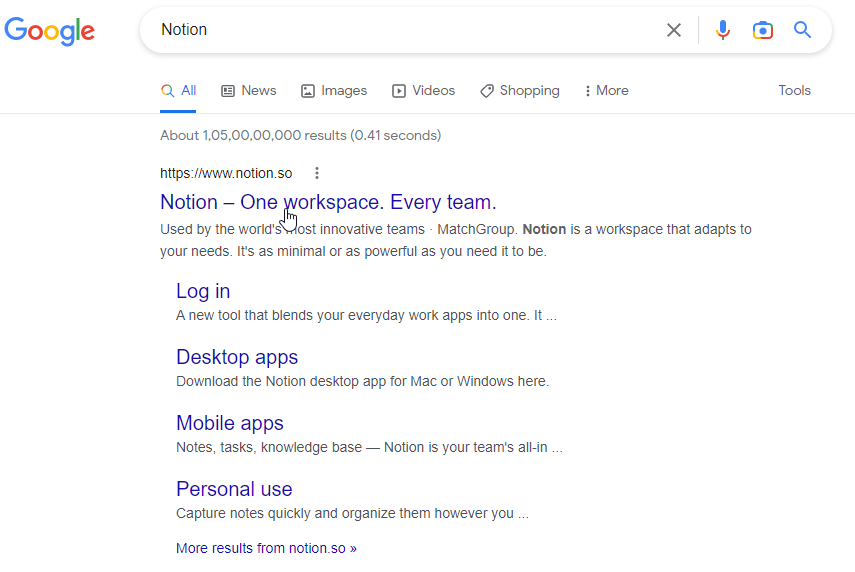
\includegraphics[scale=0.5]{gfx/1.png}
        \caption{\textbf{Click on Notion}}
        \label{fig_GN}
        \end{figure} \\
    \item On the header section, hover on \textbf{Downloads} \& select installation type as per your OS. As my PC has \textbf{Windows 10} as OS, hence I choose Windows option.
        \begin{figure}[h]
        \centering
        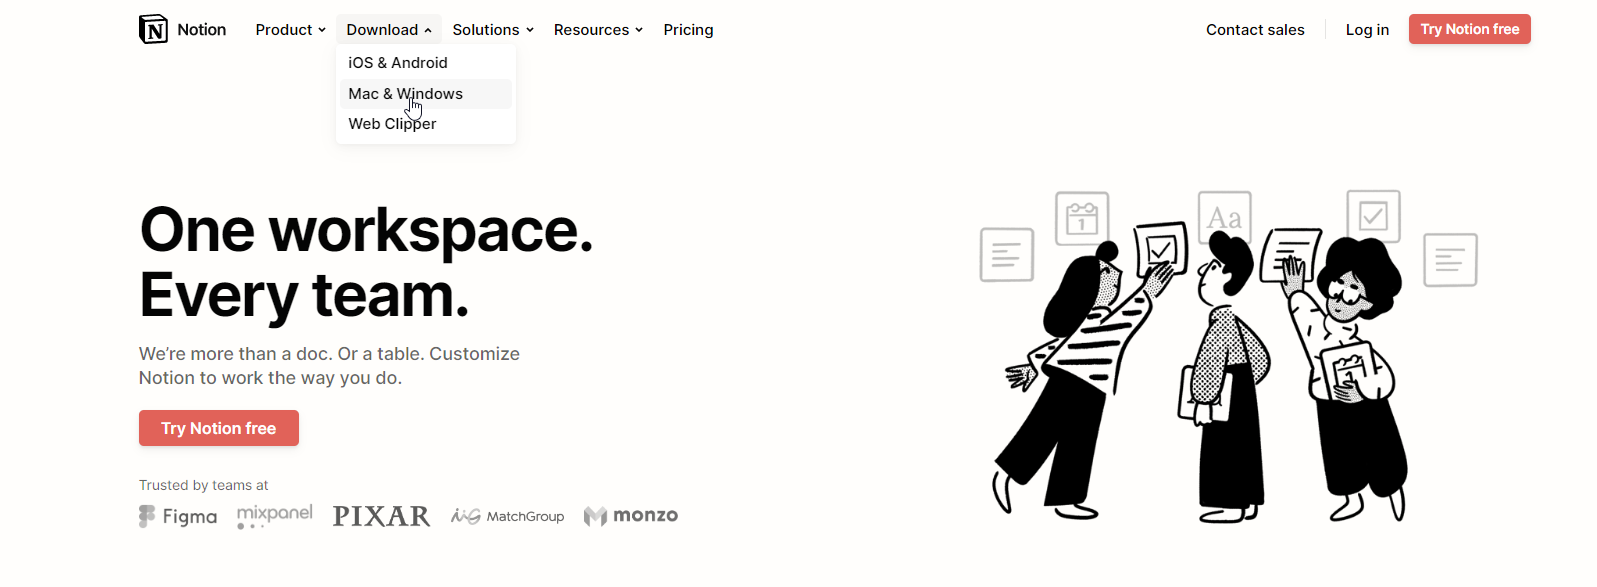
\includegraphics[scale=0.3]{gfx/2.png}
        \caption{\textbf{Click on Windows option}}
        \label{fig_GN}
        \end{figure}
    \item Now click on \textbf{Downloads for Windows} option \& it will start downloading. 
        \begin{figure}[h]
        \centering
        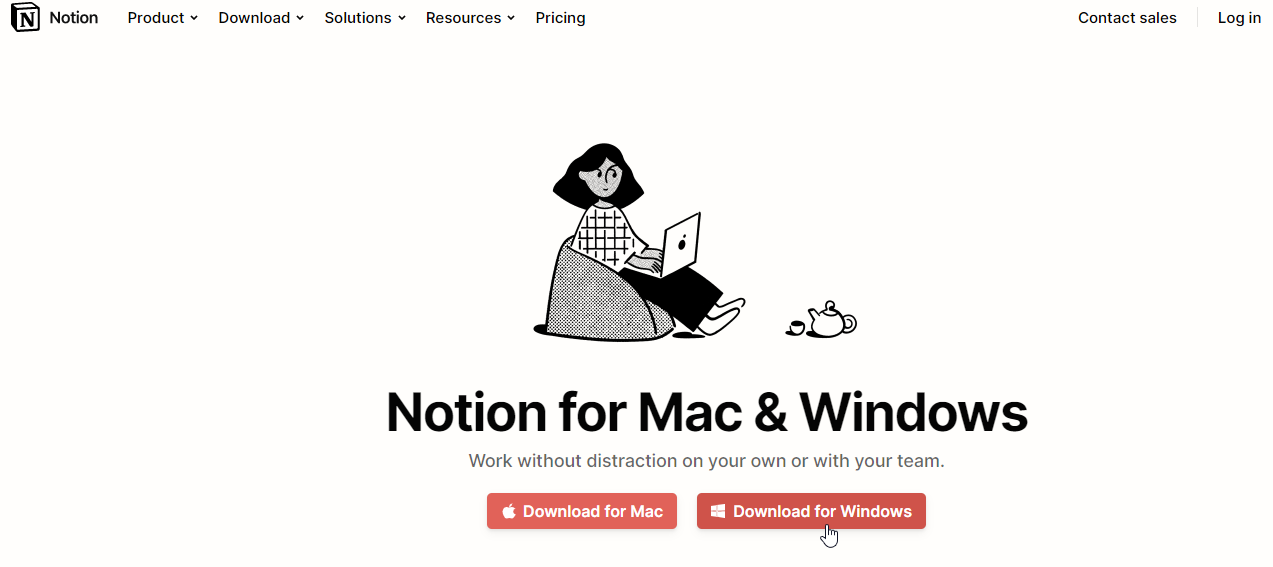
\includegraphics[scale=0.3]{gfx/3.png}
        \caption{\textbf{Downloading for Windows}}
        \label{fig_GN}
        \end{figure}
        \begin{figure}[h]
        \centering
        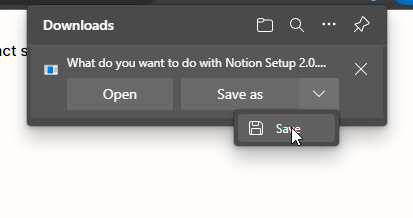
\includegraphics[scale=0.3]{gfx/4.png}
        \caption{\textbf{Downloading begins}}
        \label{fig_GN}
        \end{figure}
    \item After successful download we will begin our Installation.
        \begin{figure}[h]
        \centering
        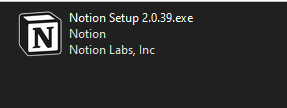
\includegraphics[scale=0.5]{gfx/5.png}
        \caption{\textbf{Notion v2.0.29 Successfully Downloaded}}
        \label{fig_GN}
        \end{figure}
\end{enumerate}
\section{Installing in Windows10}
\begin{enumerate}
    \item Right-Click on the \textbf{\textit{Notion.exe}} option \& click on \textbf{Open}.
        \begin{figure}[h]
        \centering
        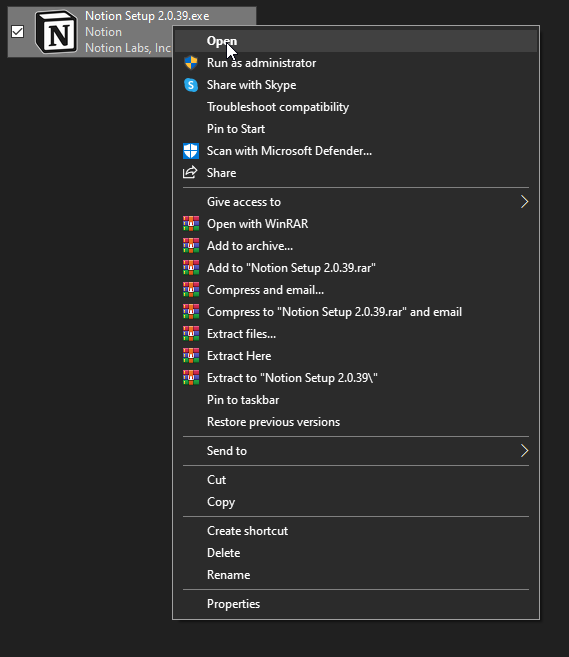
\includegraphics[scale=0.45]{gfx/6.png}
        \caption{\textbf{Clicking on Notion v2.0.29 Setup}}
        \label{fig_GN}
        \end{figure}
    \item After clicking, \textbf{\textit{Notion setup}} will get started.
        \begin{figure}[h]
        \centering
        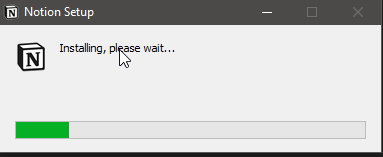
\includegraphics[scale=0.4]{gfx/7.png}
        \caption{\textbf{Installation of Notion begins}}
        \label{fig_GN}
        \end{figure}
\end{enumerate}
\newpage

% -------------------------------------- %
% -------------------------------------- %
% -------------------------------------- %


\chapter{\underline{Setting up Notion}}
\section{Signing-Up of Notion}
\begin{enumerate}
    \item Sign-up using any of the option provided. I will be using separate email-id.
        \begin{figure}[h]
        \centering
        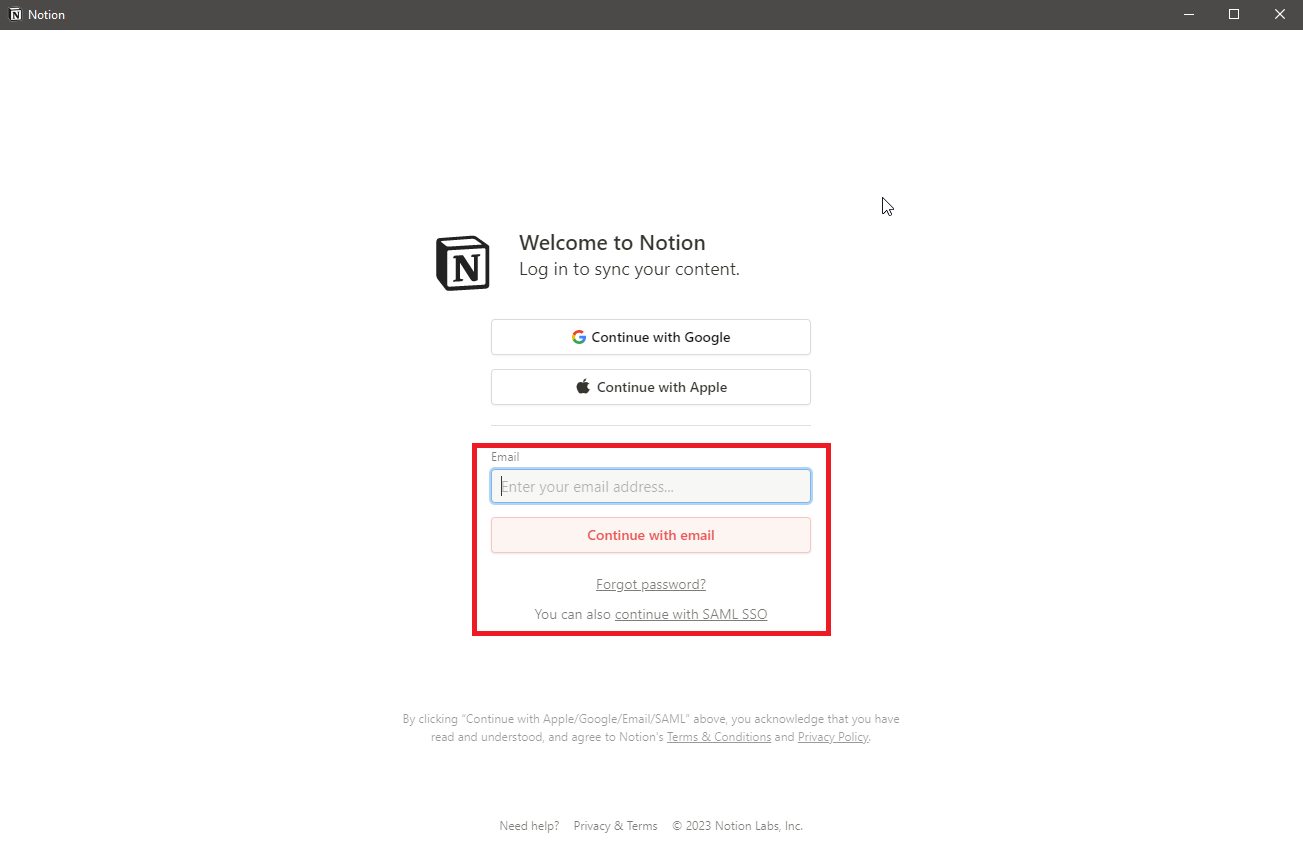
\includegraphics[scale=0.45,width=\linewidth]{gfx/8.png}
        \caption{\textbf{Sign-Up to Notion}}
        \label{fig_Sign_up_Notion}
        \end{figure} \\ \\ 
    \item As you provide valid Email-id then you will get \textbf{\textit{signup code}}, so enter it \& click on \textbf{Create New Account}.
        \begin{figure}[h]
        \centering
        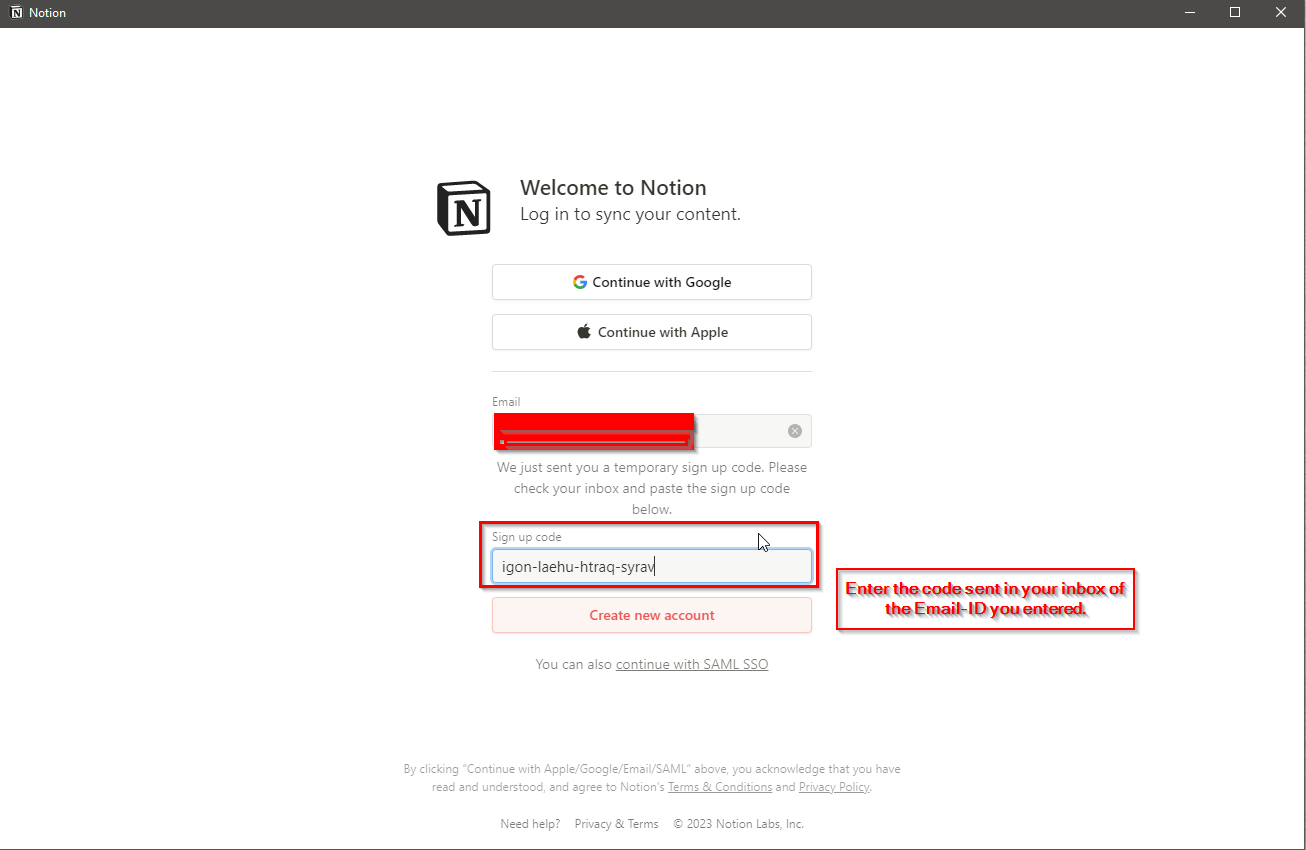
\includegraphics[scale=0.4]{gfx/9.png}
        \caption{\textbf{Entering SignUp code}}
        \label{fig: Sign_up_Code}
        \end{figure} \newpage
    \item Now put your Username \& Password along with Avatar \& click on \textbf{Continue}.
        \begin{figure}[h]
        \centering
        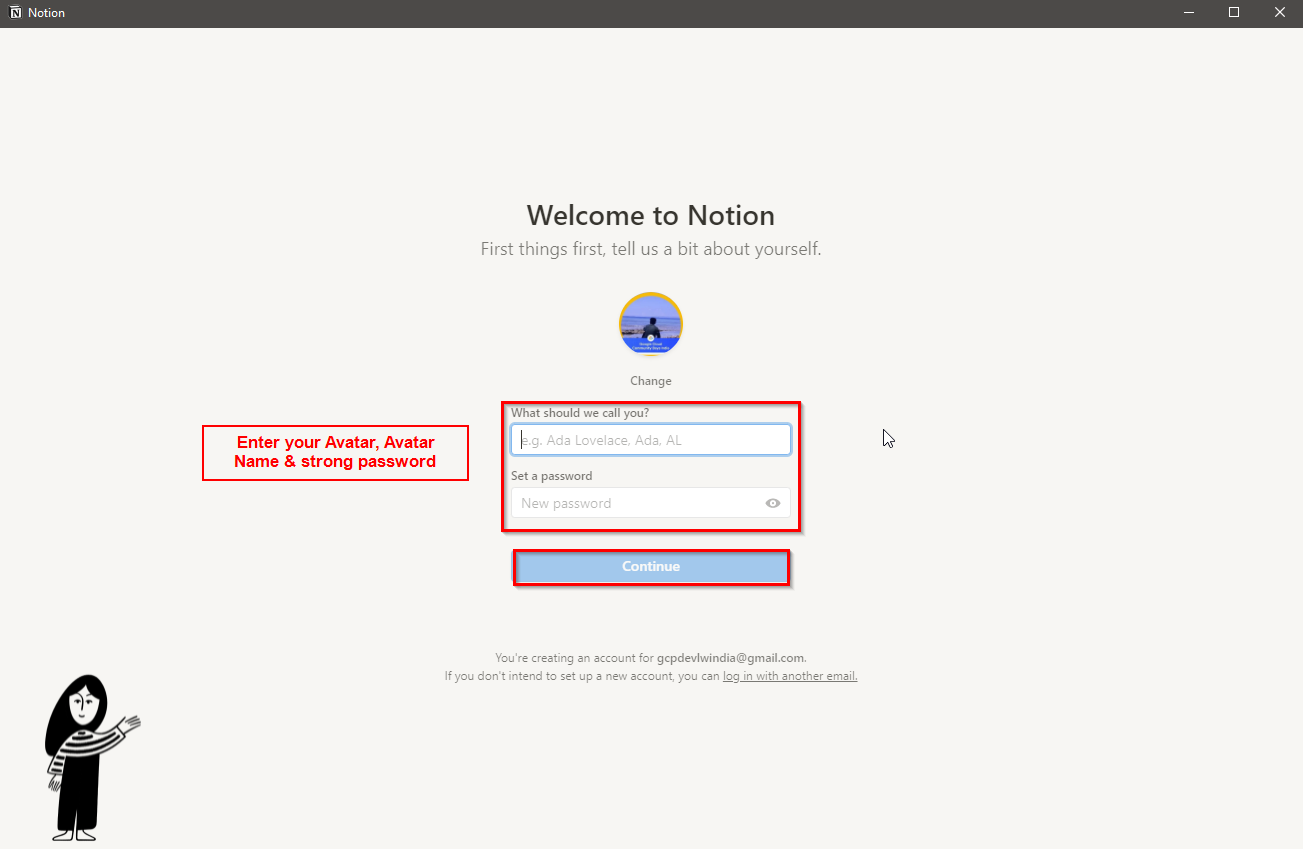
\includegraphics[scale=0.4]{gfx/10.png}
        \caption{\textbf{Setting up Credentials \& Avatar}}
        \label{fig_Sign_up_Notion}
        \end{figure}
\newpage
    \item Notion.Inc offers \textbf{Zero License Fee} for Personal use, so we will select that option. 
        \begin{figure}[h]
        \centering
        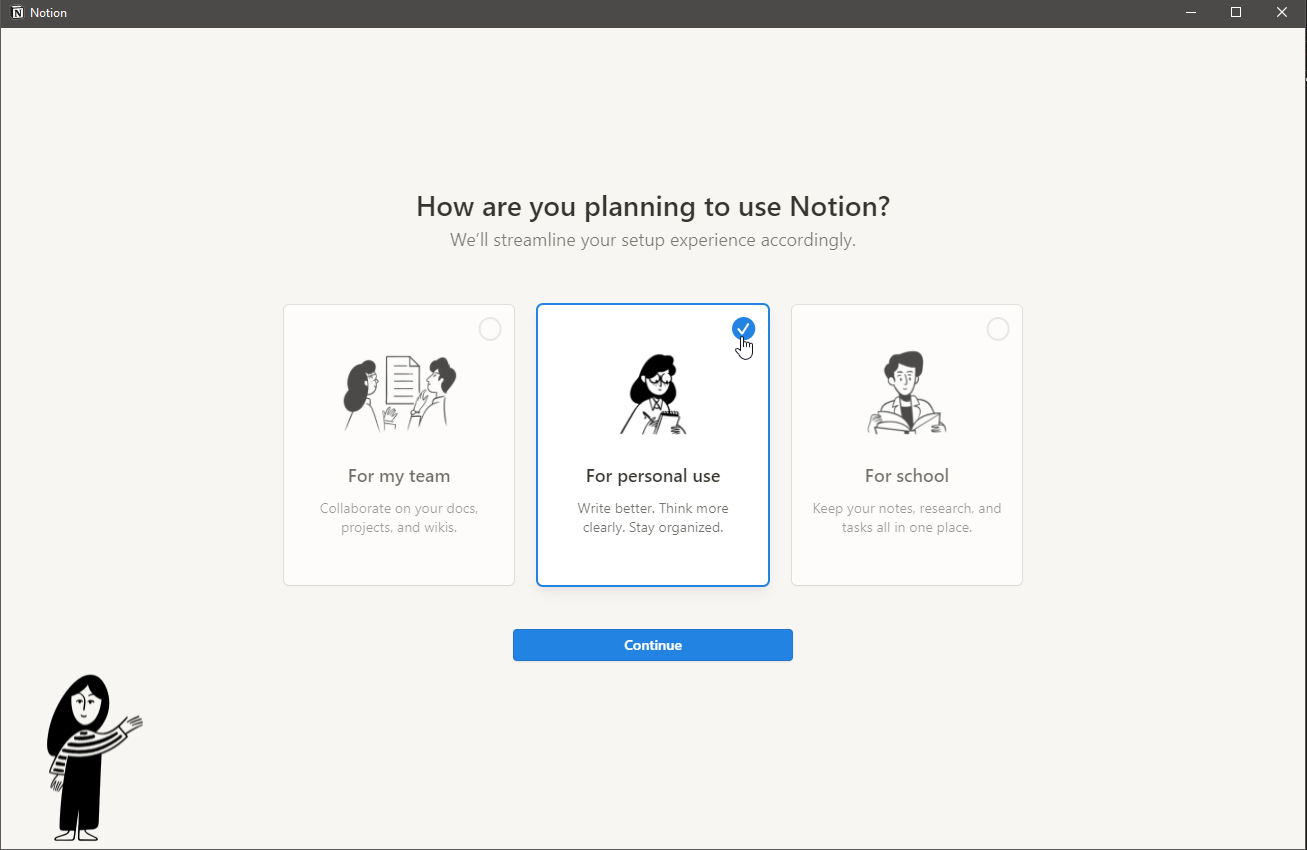
\includegraphics[scale=0.4]{gfx/11.png}
        \caption{\textbf{Selecting Mode of Use of Notion}}
        \label{fig_Sign_up_Notion}
        \end{figure} 
\newpage
    \item If you want Notion to customise itself, then provide your role or else you can simply skip it.
        \begin{figure}[h]
        \centering
        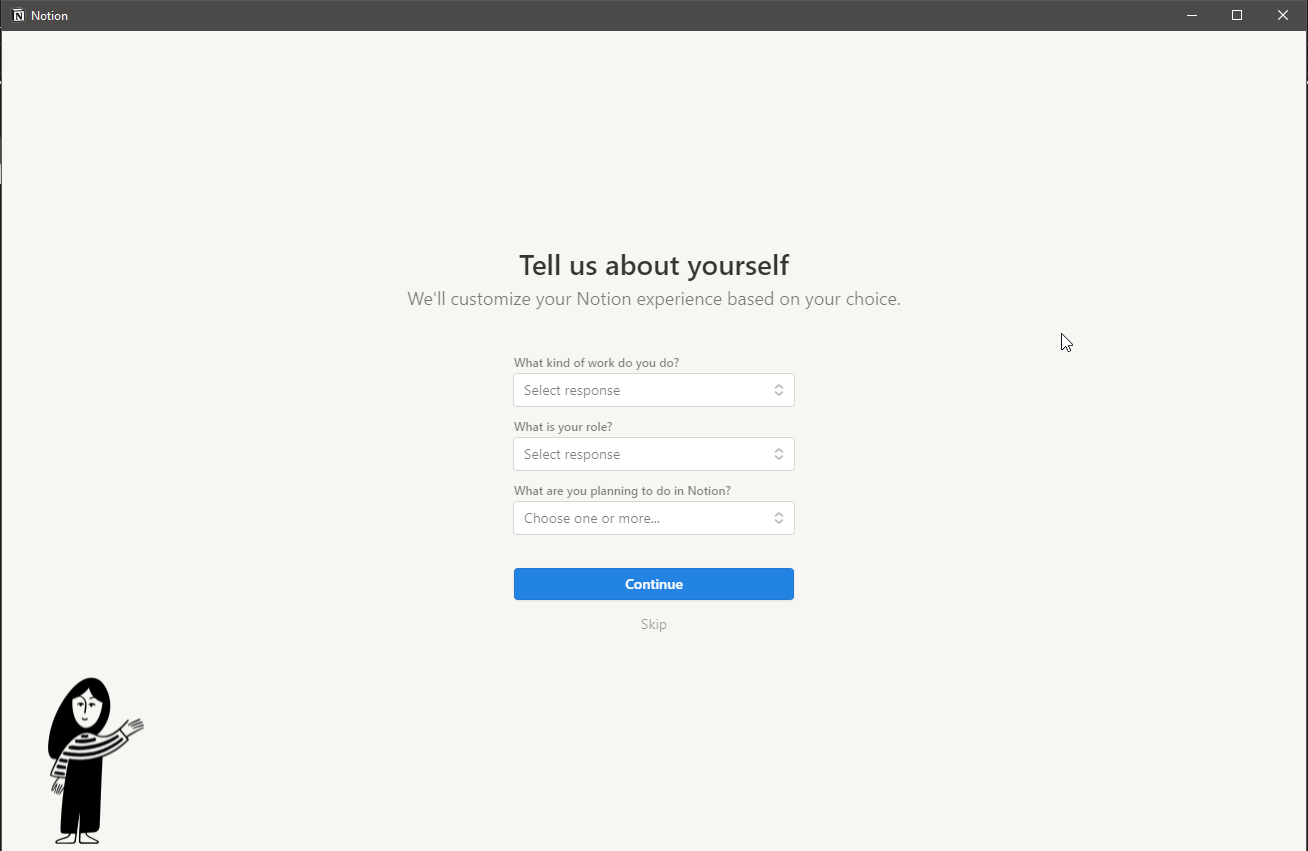
\includegraphics[scale=0.4]{gfx/12.png}
        \caption{\textbf{Customizing Notion}}
        \label{fig: Sign_up_Notion}
        \end{figure} 
\newpage
    \item Finally, your \textbf{Getting Started} page appears \& signing-up is completed.
        \begin{figure}[h]
            \centering
            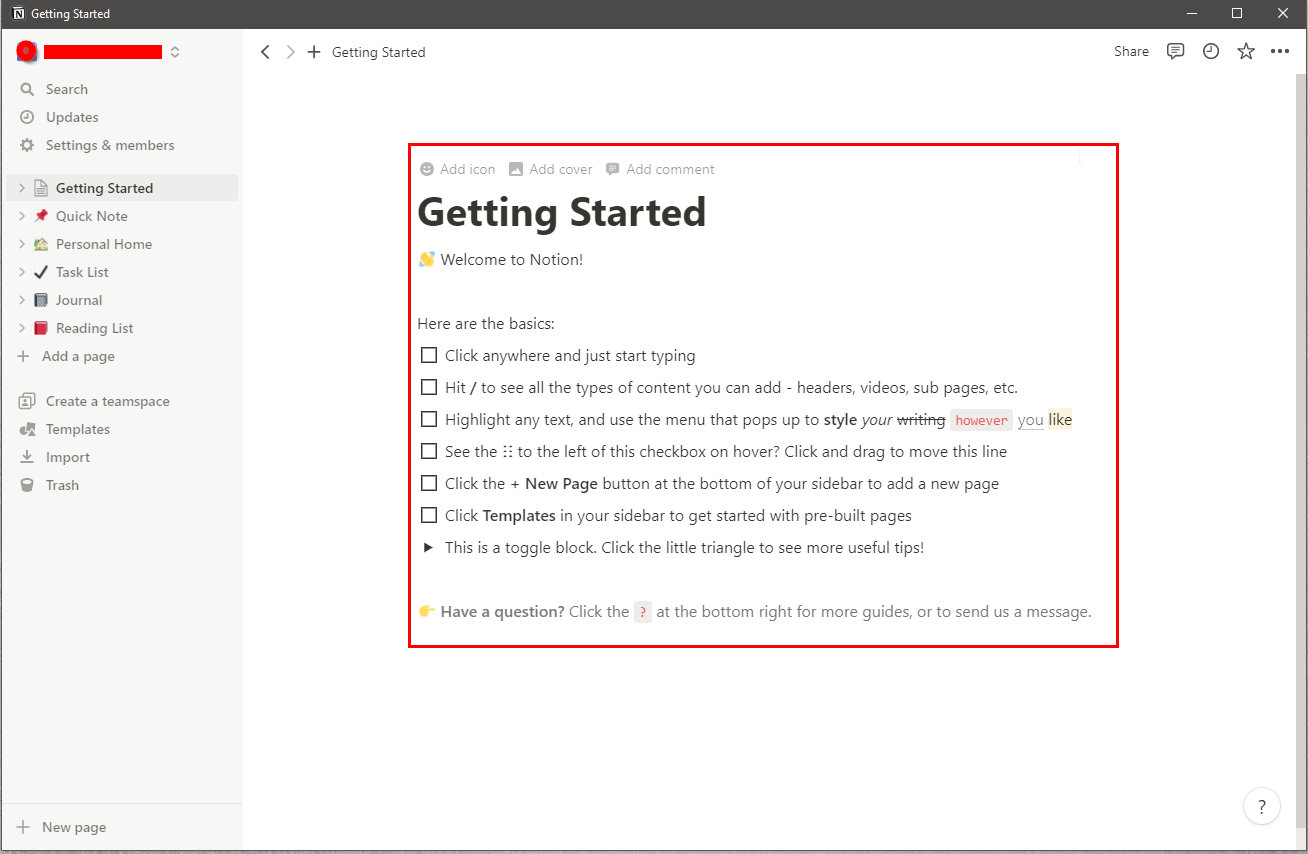
\includegraphics[scale=0.4]{gfx/13.png}
            \caption{\textbf{Getting Started Page}}
            \label{fig: Get_started}
        \end{figure}
\end{enumerate}